\usetikzlibrary{positioning, decorations.text}

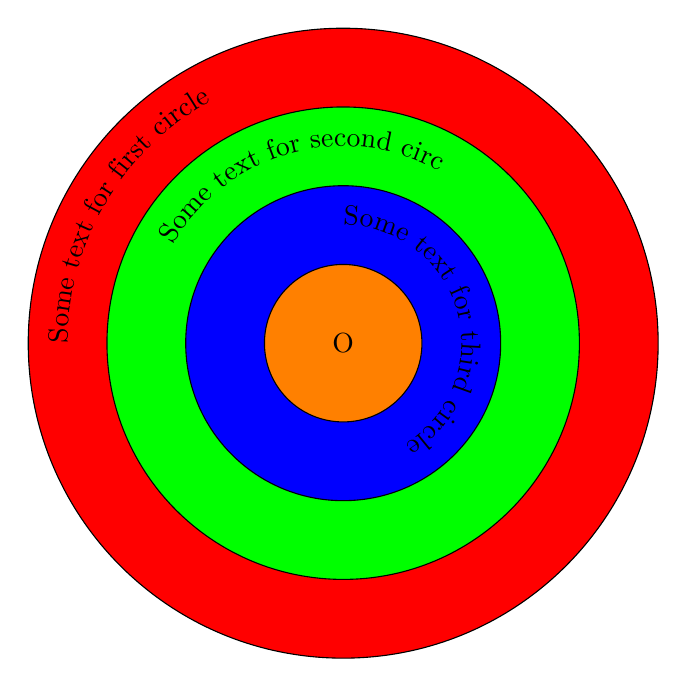
\begin{tikzpicture}

\node[circle, minimum size=8cm, draw, fill=red] (a) {};
\node[circle, minimum size=6cm, draw, fill=green] (b) {};
\node[circle, minimum size=4cm, draw, fill=blue] (c) {};
\node[circle, minimum size=2cm, draw, fill=orange] (d) {O};

\draw [decorate, decoration={text along path, text = Some text for first circle}] (180:3.5) arc (180:0:3.5cm); 

\draw [decorate, decoration={text along path, text = Some text for second circle}] (150:2.5) arc (150:60:2.5cm); 

\draw [decorate, decoration={text along path, text = Some text for third circle}] (90:1.5) arc (90:-90:1.5cm); 

\end{tikzpicture}

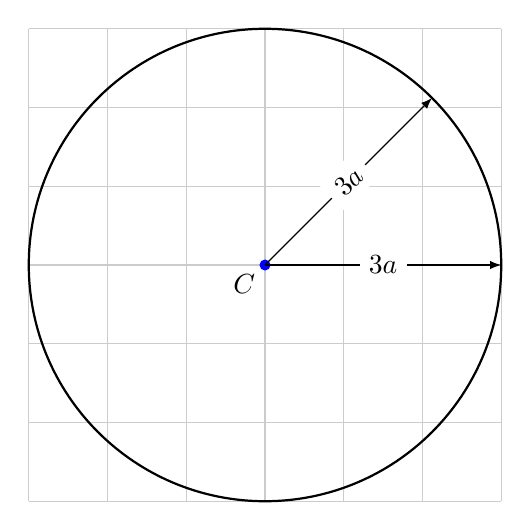
\begin{tikzpicture}[scale=1.0]

\draw [step=1.0,thin,gray!40] (0,-3) grid (6,3);

\fill[blue] (3,0) circle (2pt) node [black,below left] {$C$};
%
\draw[thick] (3,0) circle(3);
\begin{scope}[>=latex]
\draw[->] (3,0) -- (6,0)  node [midway,fill=white] {3$a$};
\draw[->] (3,0) -- ++(45:3)  node [midway,sloped,fill=white] {3$a$};
\end{scope}

\end{tikzpicture}

